\documentclass[11pt,a4paper]{article}
\usepackage[utf8]{inputenc}
\usepackage[spanish]{babel}
\usepackage{graphicx}
\usepackage{geometry}
\usepackage{booktabs}
\usepackage{listings}
\usepackage{xcolor}
\usepackage{hyperref}
\usepackage{titlesec}

% Configuración de márgenes
\geometry{top=2.5cm, bottom=2.5cm, left=2.5cm, right=2.5cm}

% Quitar la numeración automática de secciones para usar la tuya propia
\titleformat{\section}{\normalfont\Large\bfseries}{}{0pt}{}
\titleformat{\subsection}{\normalfont\large\bfseries}{}{0pt}{}
\titleformat{\subsubsection}{\normalfont\normalsize\bfseries}{}{0pt}{}

% Configuración para bloques de código de consola
\definecolor{codegray}{rgb}{0.5,0.5,0.5}
\definecolor{codeback}{rgb}{0.95,0.95,0.95}

\lstset{
    backgroundcolor=\color{codeback},
    basicstyle=\ttfamily\small,
    breaklines=true,
    commentstyle=\color{codegray},
    frame=single,
    keepspaces=true,
    numbers=none,
    showstringspaces=false,
    tabsize=2
}

% Ruta base para tus imágenes locales
\graphicspath{{./images/}}

\begin{document}

% ==========================================
% PORTADA CORPORATIVA
% ==========================================
\begin{titlepage}
    \centering
    \vspace*{2cm}
    {\Huge \bfseries [ExP 86] Entrega - Silent Exposure \par}
    \vspace{2.5cm}
    \hrule height 1pt
    \vspace{2cm}
    {\large \textbf{Entrega - Silent Exposure} \par}
    \vspace{0.6cm}
    {\large \textbf{Analista:} Xavier Margalef Riestra \par}
    \vspace{0.4cm}
    {\large \textbf{Fecha:} 2026-06-11 \par}
    \vspace{0.4cm}
    {\large \textbf{Módulo:} MF0486\_3 \par}
    \vspace{0.4cm}
    {\large \textbf{Clasificación:} Examen Práctico \par}
    \vspace{2cm}
    \hrule height 1pt
    \vfill
\end{titlepage}

% ==========================================
% BLOQUE DE CONTENIDO
% ==========================================

\subsection{Actividad 1 - Fundamentos 101}
Entrega evidencia:
\begin{center}
    
\includegraphics[width=0.50\textwidth]{image-1.png}
\end{center}

\subsection{Actividad 2 - Middle east}
Entrega evidencia:
\begin{center}
    
\includegraphics[width=0.50\textwidth]{image-4.png}
\end{center}

\subsection{Actividad 3 - Analisis 101}
Entrega evidencia:
\begin{center}
    
\includegraphics[width=0.50\textwidth]{image-6.png}
\end{center}

\newpage

\section{Actividad 4 - Silent Exposures}

\subsection{01 - Resumen Ejecutivo}
Durante la auditoría de seguridad realizada sobre la máquina \textbf{10.130.135.78 (lab-nublar-os)} se identificó una cadena de vulnerabilidades que permitió el compromiso completo del sistema.

La investigación comenzó con el análisis de servicios expuestos a través de la aplicación web, donde se \textbf{localizaron archivos de respaldo accesibles públicamente} que contenían información sensible. A partir de estos descubrimientos fue posible \textbf{obtener acceso inicial al servidor} y continuar con una fase de enumeración interna orientada a identificar configuraciones inseguras y mecanismos de escalada de privilegios.

Se detectaron controles de seguridad insuficientes relacionados con la gestión de credenciales, la exposición de información sensible y la asignación de privilegios elevados a determinados binarios del sistema. \textbf{La combinación de estas debilidades permitió obtener privilegios de administrador sobre el servidor}.

El impacto del compromiso se considera \textbf{crítico}, ya que un atacante con acceso equivalente podría consultar, modificar o eliminar información sensible, alterar la configuración del sistema, establecer mecanismos de persistencia y utilizar el servidor como punto de partida para comprometer otros activos de la infraestructura.

Como \textbf{medidas} de mitigación se recomienda:

\begin{itemize}
    \item \textbf{Saneamiento de activos}: Eliminar permanentemente archivos de desarrollo y copias de respaldo de los entornos productivos.
    \item \textbf{Refuerzo de controles}: Aplicar el principio de mínimo privilegio y auditar binarios con permisos elevados (SUID), reduciendo así la superficie de ataque.
    \item \textbf{Gestión de credenciales}: Reforzar la política de acceso y rotar las llaves comprometidas para restaurar la cadena de confianza.
    \item \textbf{Ciclo de mejora}: Establecer revisiones periódicas que aseguren la trazabilidad de los eventos, garantizando que el sistema vuelva a ser una fuente confiable dentro de la infraestructura corporativa.
\end{itemize}

\newpage

\subsection{02 - Fase de Reconocimiento}
El objetivo de esta fase es \textbf{verificar la disponibilidad del servidor, identificar servicios activos y analizar la configuración del servidor web}.

\subsubsection{2.1 Identificación del objetivo}
\begin{itemize}
    \item Dirección IP del servidor: \textbf{10.130.135.78}
\end{itemize}

\subsubsection{2.2 Verificación de conectividad}
Se comprobó que el servidor estaba operativo mediante un ping:
\begin{lstlisting}[language=bash]
ping 10.130.135.78
\end{lstlisting}
\begin{center}
    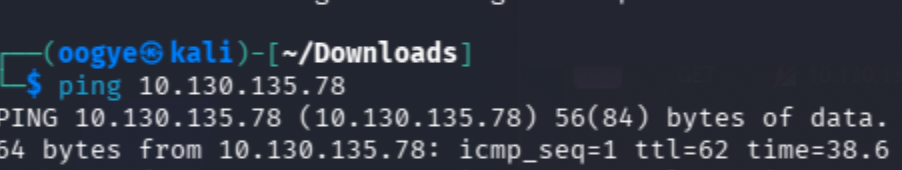
\includegraphics[width=0.75\textwidth]{image-26.png}
\end{center}

\subsubsection{2.3 Acceso y análisis web inicial}
\begin{itemize}
    \item Se accedió a la IP mediante navegador.
    \item Se utilizaron \textbf{Dev Tools} para inspeccionar HTTP, puerto y estructura HTML.
\end{itemize}

\textbf{Hallazgos:}
\begin{itemize}
    \item Protocolo: \textbf{HTTP}
    \begin{center}
        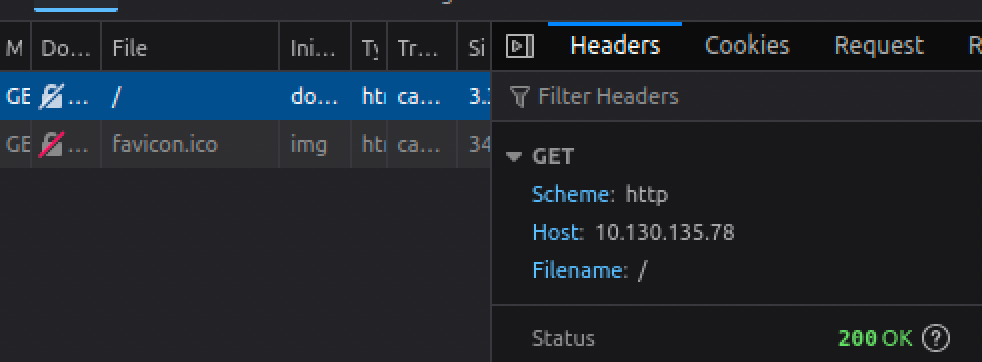
\includegraphics[width=0.55\textwidth]{image-22.png}
    \end{center}
    \item Puerto: \textbf{80} (\href{https://stackoverflow.com/questions/3364144/is-port-number-required-in-http-host-header-parameter}{referencia})
    \item Título de página en \texttt{<title>}:
    \begin{center}
        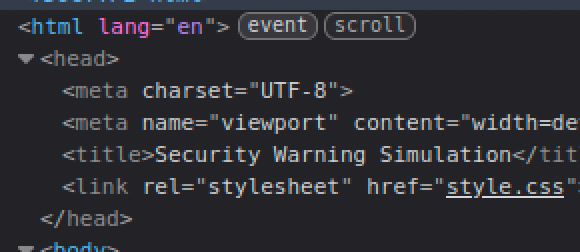
\includegraphics[width=0.55\textwidth]{image-23.png}
    \end{center}
    \item Código de error y motivo mediante opciones avanzadas:
    \begin{center}
        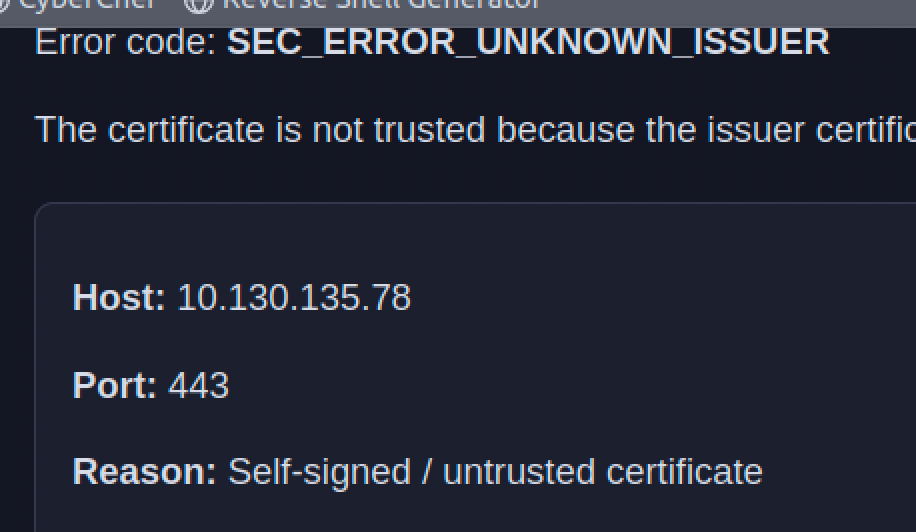
\includegraphics[width=0.55\textwidth]{image-24.png}
    \end{center}
\end{itemize}

\subsubsection{2.4 Descarga de archivo de prueba}
\begin{itemize}
    \item Se aceptaron riesgos y se descargó el archivo disponible.
    \item Contenía la flag: \textbf{"Bienvenidos a Jurassic Park"}
\end{itemize}
\begin{center}
    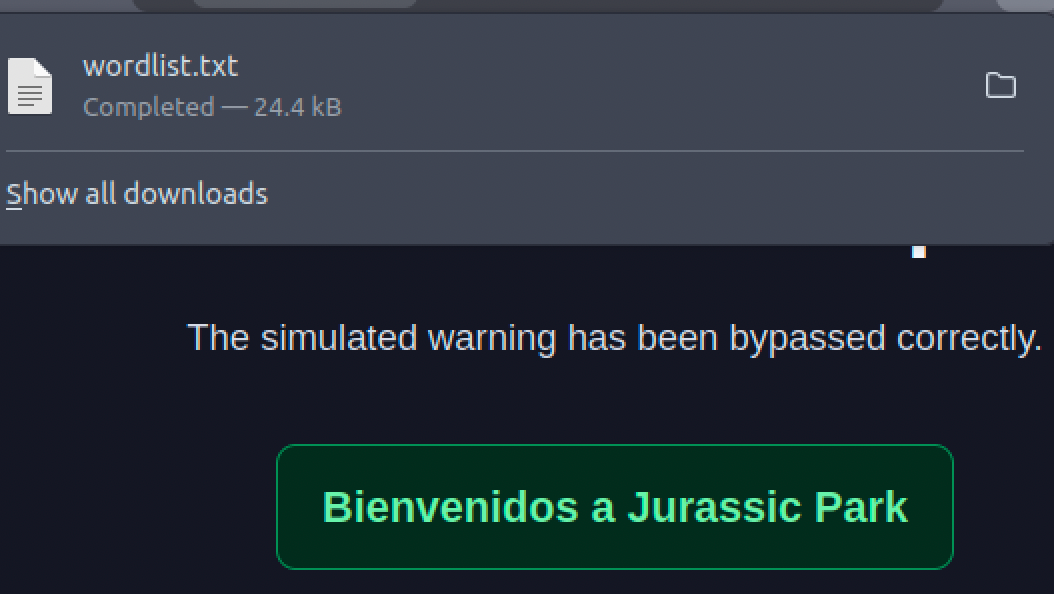
\includegraphics[width=0.55\textwidth]{image-25.png}
\end{center}
Archivo en texto plano, útil para fases posteriores.\\
Relevancia del uso de wordlists: \href{https://www.freecodecamp.org/news/the-power-of-wordlists-why-every-ethical-hacker-needs-one/}{FreeCodeCamp}

\newpage

\subsection{03 - Fase de Enumeración y Descubrimiento}
Realizamos una fase de enumeración de directorios y archivos para identificar rutas ocultas en el servidor web. El objetivo es localizar recursos no indexados o expuestos que puedan servir como vector de ataque.

\subsubsection{3.1 Enumeración de directorios y archivos}
Se utilizó \textbf{fuzzing} y \textbf{fuerza bruta} para identificar rutas ocultas o archivos sensibles.
\begin{lstlisting}[language=bash]
dirb http://10.130.191.20 /root/wordlist.txt/
gobuster dir -u http://10.130.191.20 -w /root/wordlist.txt
dirb http://10.129.175.105 /root/wordlist.txt -N 403
\end{lstlisting}

\begin{itemize}
    \item \texttt{dirb} nos devuelve que hay 17 archivos en el servidor:
    \begin{center}
        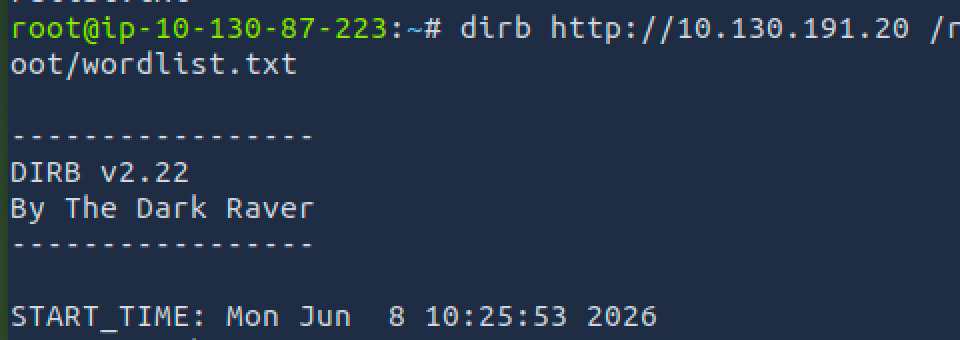
\includegraphics[width=0.75\textwidth]{image-28.png}
    \end{center}
    \item \texttt{Gobuster} nos da más detalles como la respuesta en el acceso a los archivos (especificando los \textbf{200 y 403}):
    \begin{center}
        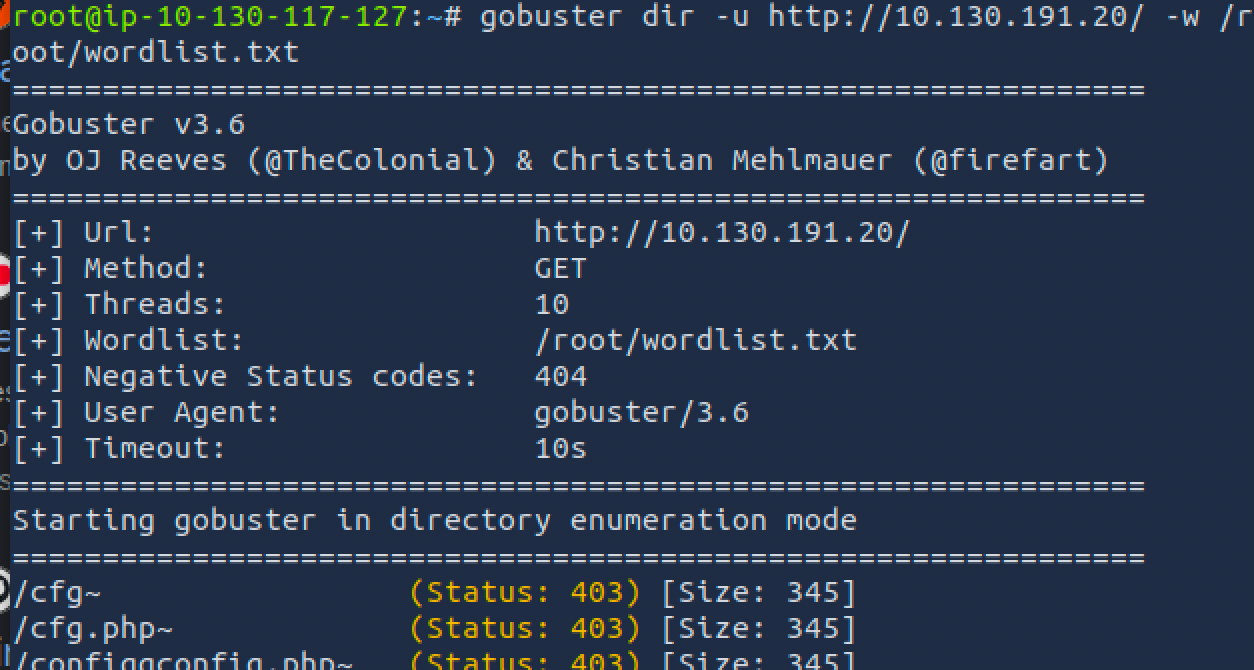
\includegraphics[width=0.75\textwidth]{image-29.png}
    \end{center}
\end{itemize}

Para filtrar los archivos con respuesta negativa como el 403, añadimos \texttt{-N 403} al final del dirb:
\begin{center}
    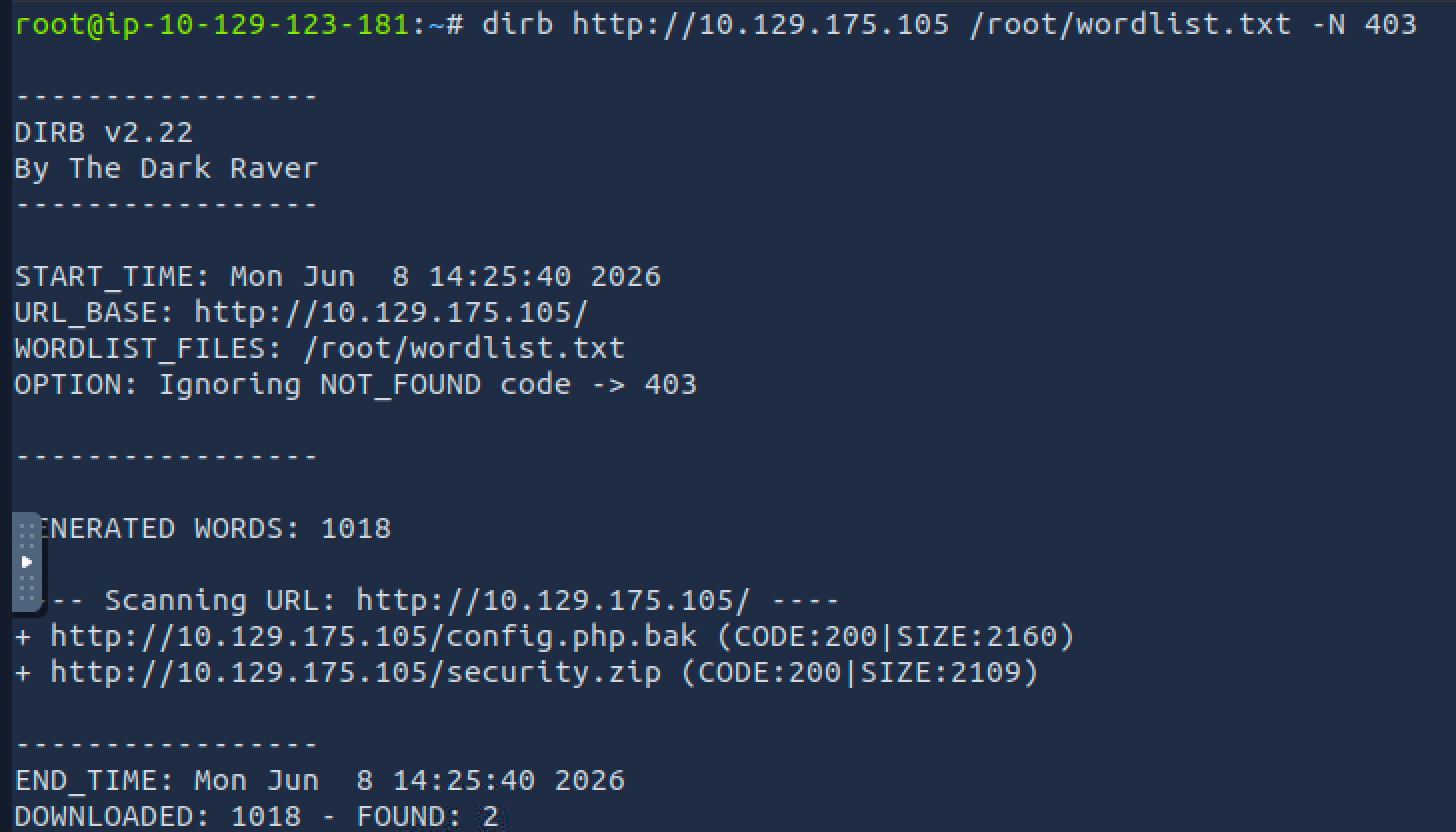
\includegraphics[width=0.75\textwidth]{image-30.png}
\end{center}
Este comando fue encontrado en una guía de \href{https://www.linkedin.com/pulse/dirb-cyberhorizon-defentech-zo21c}{LinkedIn} dado que otras \textbf{opciones como -b o -x o -s no funcionaban.}

\begin{itemize}
    \item Archivos descubiertos: \texttt{config.php.bak} y \texttt{security.zip}
\end{itemize}
\begin{center}
    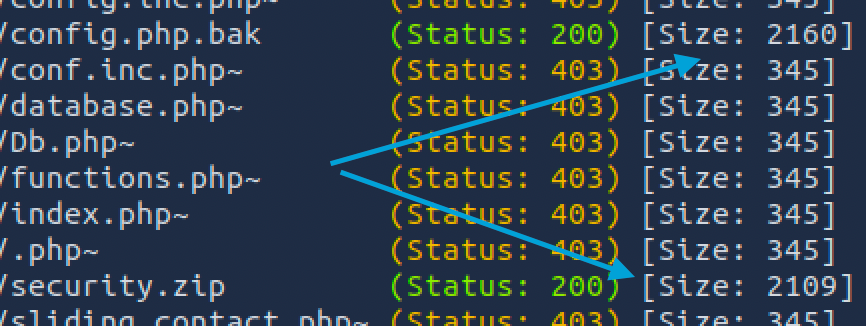
\includegraphics[width=0.65\textwidth]{image-39.png}
\end{center}

Por el momento nos encontramos delante de una vulnerabilidad que afecta a la confidencialidad debido a que usuarios no autorizados acceden a información privilegiada crítica para el sistema con dos archivos con estatus 200.

\subsubsection{3.2 Análisis de archivos críticos}
Identificamos mediante un comando grep información clave como el nombre de la intranet o el host con \texttt{grep "host" wordlist.txt} que nos devuelve que el host es \textbf{localhost}:
\begin{center}
    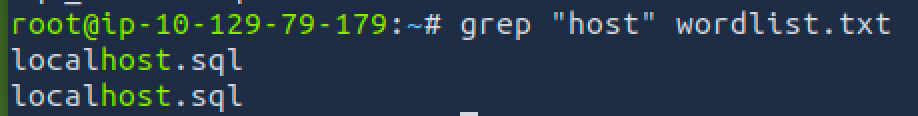
\includegraphics[width=0.7\textwidth]{image-35.png}
\end{center}
Para identificar el nombre de la intranet no encontramos ningún archivo con \texttt{grep} analizando el \texttt{wordlist.txt}:
\begin{center}
    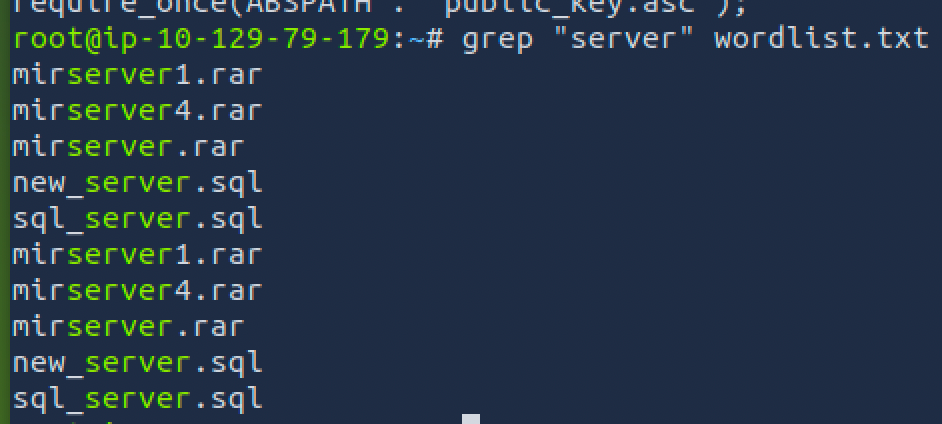
\includegraphics[width=0.7\textwidth]{image-34.png}
\end{center}
Así que tenemos que ir más abajo ya que es la información accesible más directa que tenemos para explorar los dos archivos que nos devuelve gobuster como accesibles con 200 status code que son \textbf{config.php.bak} y \textbf{security.zip}.

\paragraph{config.php.bak}

Como es un \textbf{backup} de un archivo importante y probablemente tenga información sobre el servidor y la base de datos. Buscando cómo descargarse archivos después de identificarlos con gobuster de este \href{https://infosecwriteups.com/how-to-use-gobuster-to-find-interesting-directories-files-on-website-a1aaf8fc771e?gi=44e8bf222dde}{write up} encontramos que el comando es \texttt{wget}:
\begin{lstlisting}[language=bash]
wget http://10.129.175.105/config.php.bak
cat config.php.bak
\end{lstlisting}
\begin{center}
    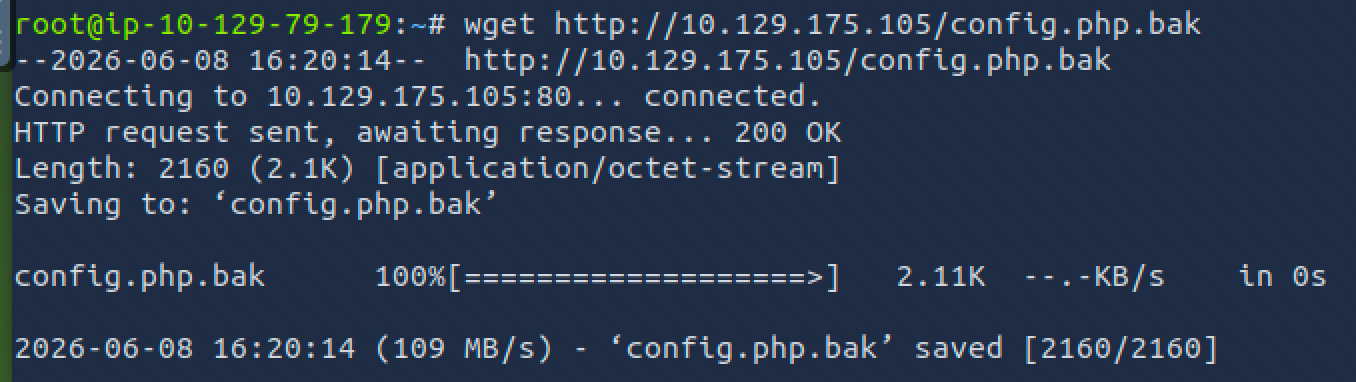
\includegraphics[width=0.48\textwidth]{image-36.png}\hfill
    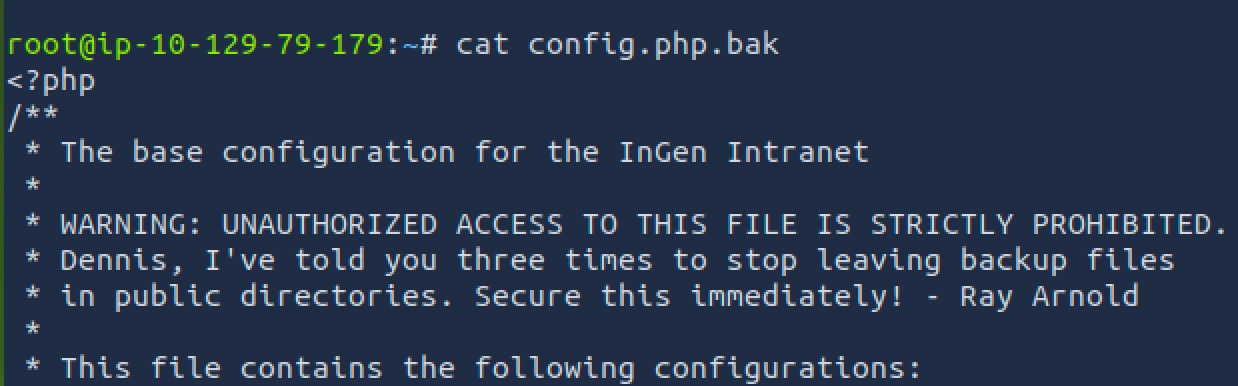
\includegraphics[width=0.48\textwidth]{image-37.png}
\end{center}

\begin{itemize}
    \item Intranet: \texttt{ingen\_park\_ops}
    \item Codificación: \texttt{utf8mb4}
    \item Auth keys, prefijo de base de datos y clave del parque:
\end{itemize}
\begin{center}
    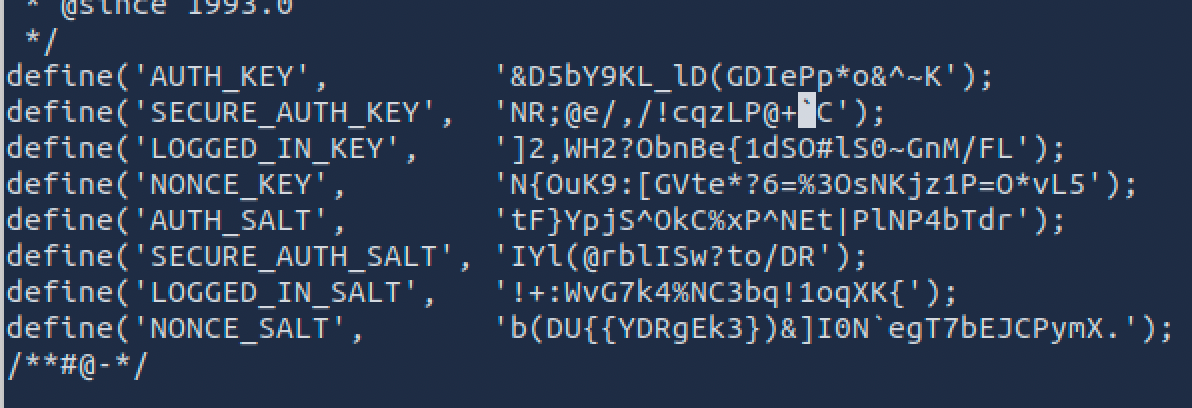
\includegraphics[width=0.48\textwidth]{image-33.png}\hfill
    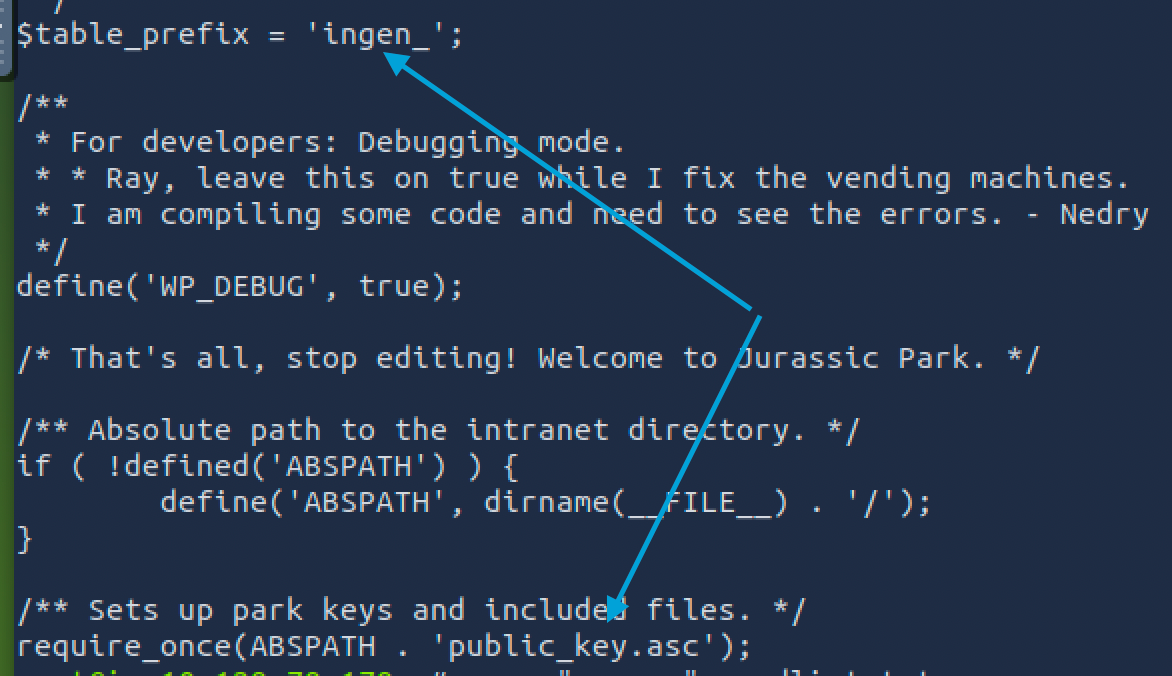
\includegraphics[width=0.48\textwidth]{image-38.png}
\end{center}

\paragraph{security.zip}
\begin{lstlisting}[language=bash]
wget http://10.129.175.105/security.zip
\end{lstlisting}
\begin{itemize}
    \item Contenido protegido con contraseña obtenida de \texttt{config.php.bak}:
    \begin{center}
        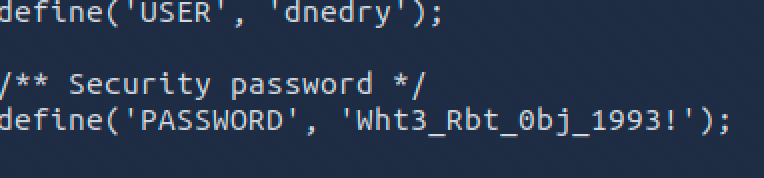
\includegraphics[width=0.55\textwidth]{image-40.png}
    \end{center}
    \item Llave pública \texttt{public\_key.asc} (GPG, RSA 3072 bits):
    \begin{center}
        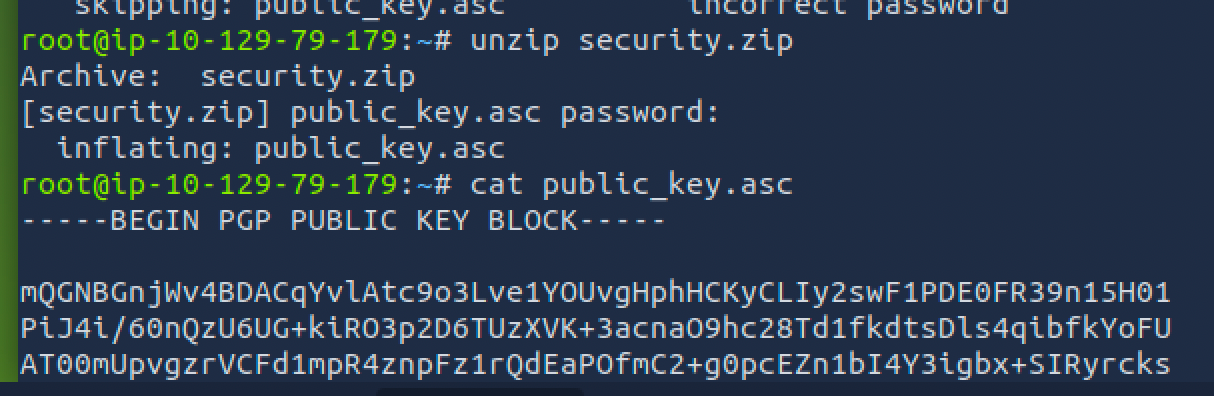
\includegraphics[width=0.48\textwidth]{image-41.png}\hfill
        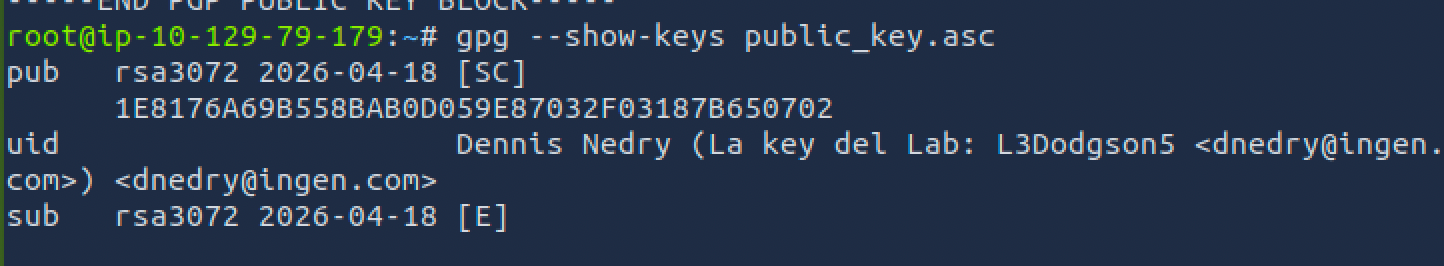
\includegraphics[width=0.48\textwidth]{image-42.png}
    \end{center}
\end{itemize}

Esta extracción es muy importante porque esto nos da la llave de acceso para conectarnos al servidor web ya que es GPG, que es una herramienta que utiliza el sistema de claves públicas y privadas para comunicar entre aplicaciones mediante \textbf{SSH}.

Para averiguar qué algoritmo de cifrado usa para cifrar la clave pública, debemos aplicar el comando \texttt{gpg --show-keys public\_key.asc} que nos devuelve que usa RSA de 3072 bits. Esto lo encontramos investigando más sobre \href{https://www.gnupg.org/gph/es/manual.html}{GNU}.

\newpage

\subsection{04 - Fase de Acceso Inicial y Análisis del Sistema}
Una vez obtenido acceso al sistema mediante credenciales válidas, se inicia una fase de enumeración interna con el objetivo de comprender la arquitectura del servidor, identificar usuarios relevantes, analizar los servicios en ejecución y detectar posibles configuraciones vulnerables que pudieran facilitar una escalada de privilegios.

\subsubsection{4.1 Acceso SSH}
Accedemos con SSH al host del servidor, pasando de ser un usuario externo a un usuario interno con acceso directo a la consola del servidor. A esto le llamamos \href{https://www.incibe.es/incibe-cert/blog/acceso-inicial-no-autorizado-equipos-sci-parte-1}{Intrusión o Acceso Inicial / Pivoteo}.
\begin{lstlisting}[language=bash]
ssh dnedry@10.129.175.105
\end{lstlisting}
\begin{center}
    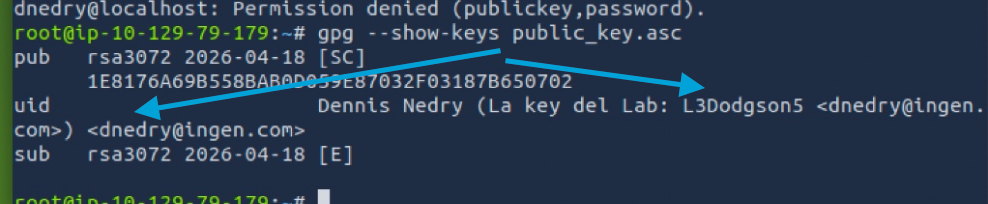
\includegraphics[width=0.48\textwidth]{image-44.png}\hfill
    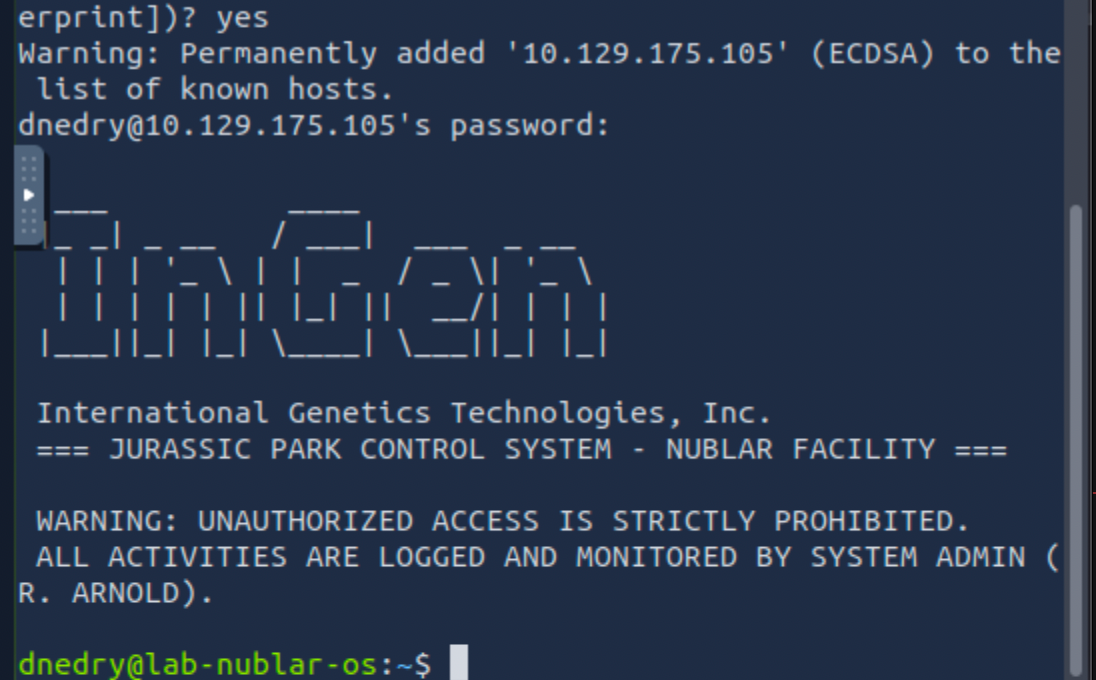
\includegraphics[width=0.48\textwidth]{image-45.png}
\end{center}

\begin{itemize}
    \item Directorio inicial: \texttt{/home/dnedry} identificado con \texttt{pwd}:
    \begin{center}
        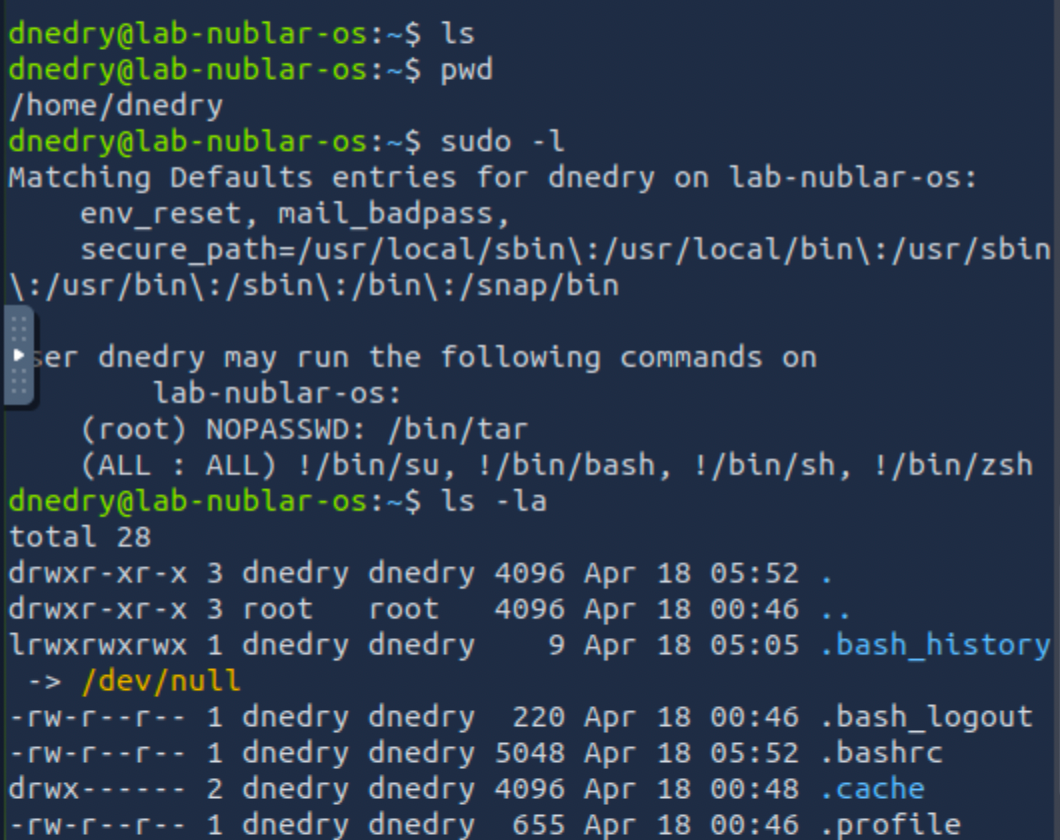
\includegraphics[width=0.5\textwidth]{image-46.png}
    \end{center}
    \item Usuarios en el sistema: 28 con \texttt{awk -F ":" '\{print \$1\}' /etc/passwd} encontrado en \href{https://man7.org/linux/man-pages/man5/passwd.5.html}{Man7}:
    \begin{center}
        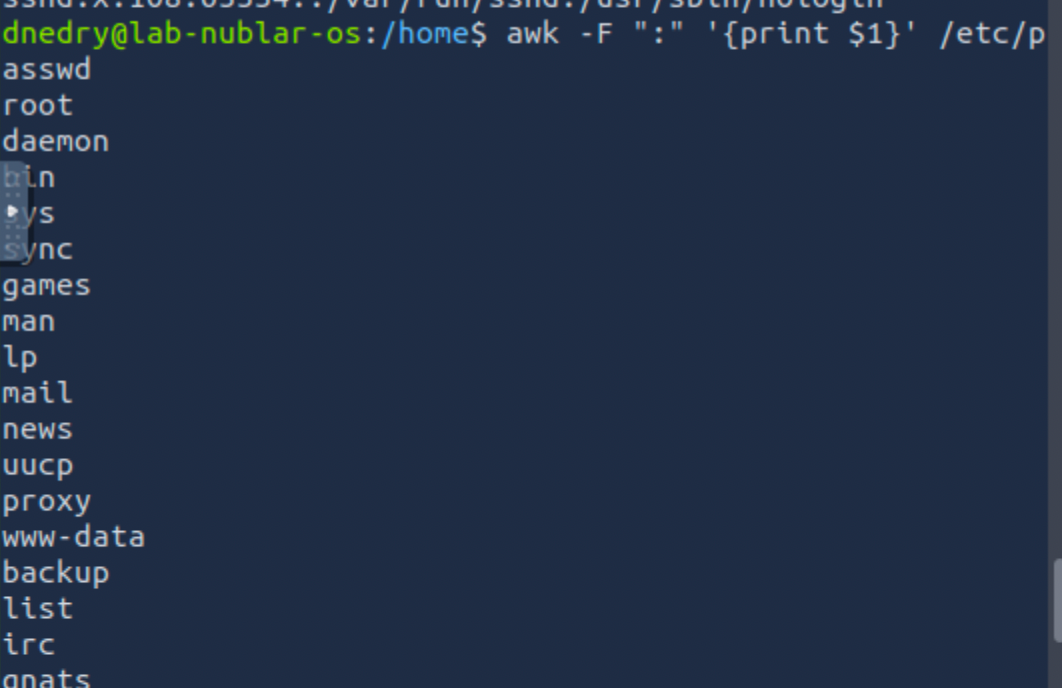
\includegraphics[width=0.55\textwidth]{image-49.png}
    \end{center}

    \item Usuario principal de monitoreo: R.ARNOLD:
    \begin{center}
        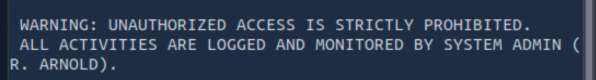
\includegraphics[width=0.5\textwidth]{image-50.png}
    \end{center}

    \item Hostname: \texttt{lab-nublar-os}:
    \begin{center}
        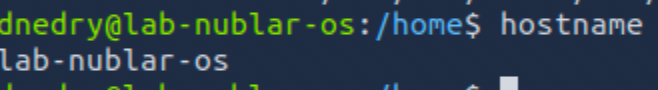
\includegraphics[width=0.5\textwidth]{image-51.png}
    \end{center}

    \item Distribución: \texttt{securityos} identificado con \texttt{cat /etc/os-release}:
    \begin{center}
        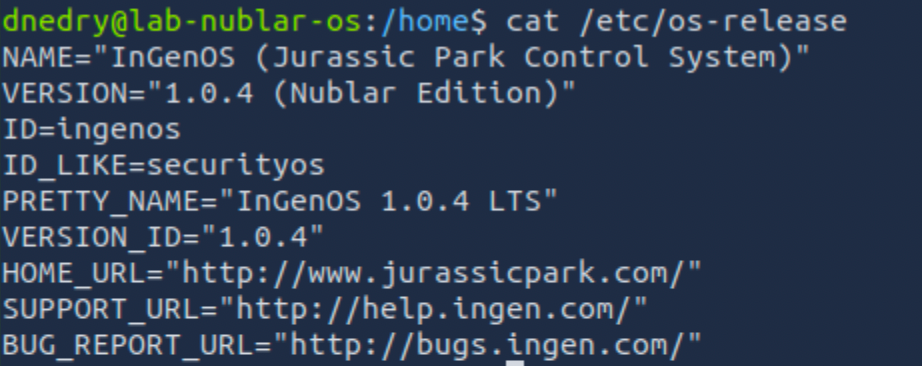
\includegraphics[width=0.55\textwidth]{image-52.png}
    \end{center}

    \item Grupos del usuario:
    \begin{center}
        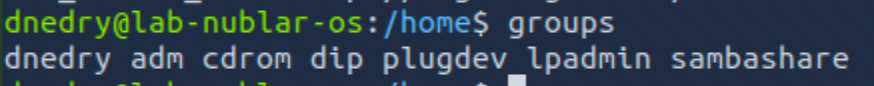
\includegraphics[width=0.5\textwidth]{image-53.png}
    \end{center}
\end{itemize}

\subsubsection{4.2 Puertos y servicios}
Ahora necesitamos hacer un análisis de la red del servidor, empezando por mirar cómo chequear qué puertos están abiertos en el servidor linux buscando en \href{https://docs.redhat.com/es/documentation/red_hat_enterprise_linux/6/html/security_guide/sect-security_guide-server_security-verifying_which_ports_are_listening}{Red Hat Documentation} donde encontramos que \texttt{nmap + IP} nos indica los puertos abiertos pero al intentar tirarlo nos da error de que no está instalado:
\begin{center}
    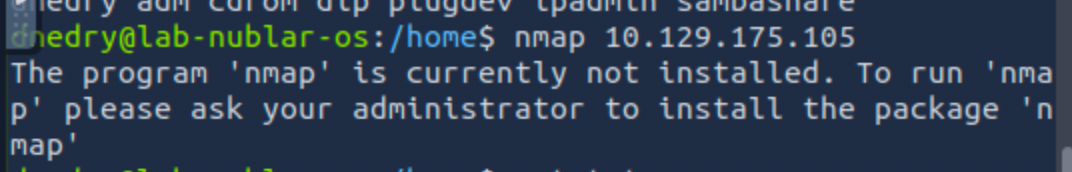
\includegraphics[width=0.6\textwidth]{image-54.png}
\end{center}

Haciendo una búsqueda concreta de \textbf{check open ports linux} encontramos en \href{https://superuser.com/questions/529830/get-a-list-of-open-ports-in-linux}{SuperUser} que un comando mejor es \texttt{netstat -lntu} porque las flags utilizadas aplican los filtros exactos a nivel de kernel, eliminando todo el ruido sin necesidad de usar grep, garantizando una visibilidad real de los sockets abiertos y reduciendo la posibilidad de falsos positivos en la enumeración de puertos.
\begin{lstlisting}[language=bash]
netstat -lntu
\end{lstlisting}
    \item 4 puertos abiertos:
\end{itemize}
\begin{center}
    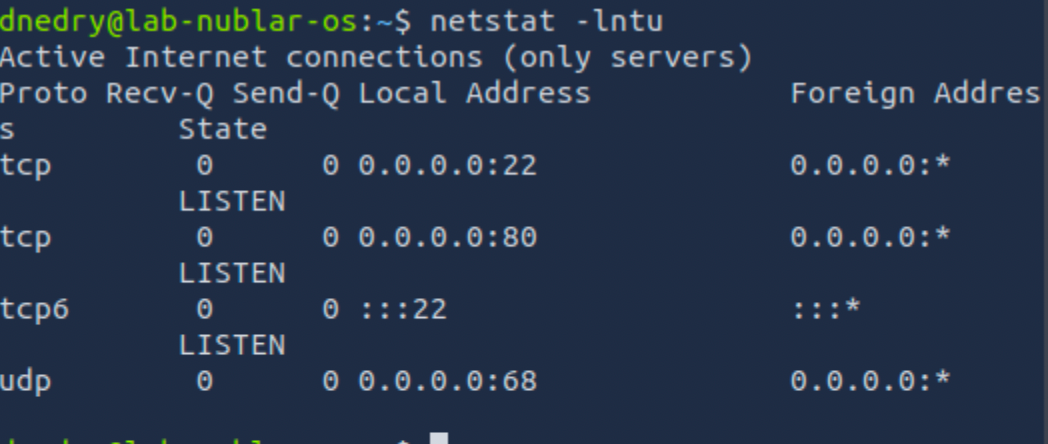
\includegraphics[width=0.7\textwidth]{image-57.png}
\end{center}

\subsubsection{4.3 Espacio en disco}
Seguimos analizando unidades del sistema y ahora buscamos porcentaje de disco usado por el sistema. Buscamos en Google para encontrar una \href{https://terminaldelinux.com/terminal/disco/espacio-libre-usado/}{explicación del porqué} y encontramos que \texttt{df -h} nos informa del espacio libre en cada partición del disco.

En el disco encontramos \textbf{18GB} disponibles. Para resolver el reto ignoramos el valor de 17G que mostraba el comando \texttt{df -h} porque \href{https://man7.org/linux/man-pages/man1/df.1.html}{Linux calcula en base 2 (Gibibytes)}, y ejecutamos \texttt{df -B 1 /} para obtener los bytes puros disponibles (17.302.560.768 bytes); al aplicar la pista de potencias de 10 ($10^9$) dividiendo entre mil millones, obtenemos 17,3 GB, valor que el sistema redondea al alza dando el número 18.
\begin{lstlisting}[language=bash]
df -h
\end{lstlisting}
\begin{itemize}
    \item Porcentaje de disco usado: 009\%
    \item Espacio disponible: 18 GB
\end{itemize}
\begin{center}
    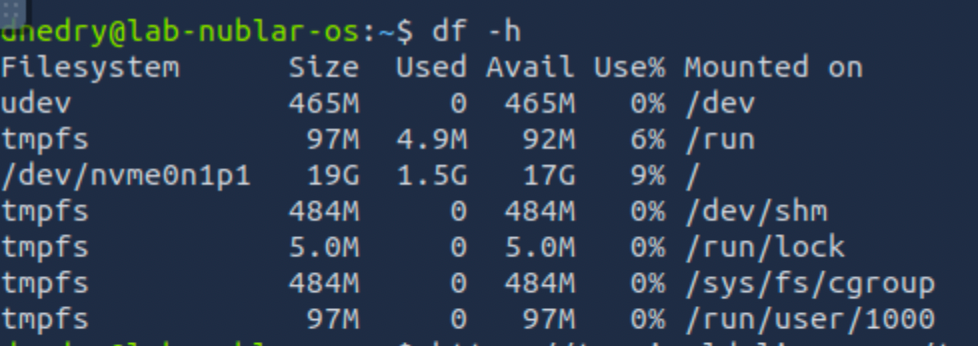
\includegraphics[width=0.7\textwidth]{image-58.png}
\end{center}

\subsubsection{4.4 Información sobre usuario www-data}
Ahora vamos a buscar información sobre \textbf{www-data} que es el usuario estándar en sistemas Linux que utiliza el servidor web para ejecutarse y gestionar los archivos de las páginas de forma aislada y segura.

Para extraerla y verla en pantalla, ejecutamos según lo encontrado en \href{https://stackoverflow.com/questions/57245919/how-to-check-which-user-a-certain-process-belongs-to}{Stack-Overflow}:
\begin{lstlisting}[language=bash]
ps aux | grep www-data
\end{lstlisting}
\begin{itemize}
    \item Ruta y usuario www-data: \textbf{ruta /usr/sbin/lighttpd -D -f /etc/lighttpd/lighttpd.conf}
\end{itemize}
\begin{center}
    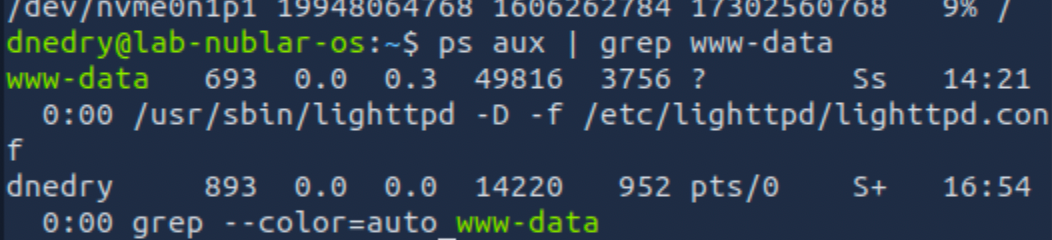
\includegraphics[width=0.75\textwidth]{image-60.png}
\end{center}

\subsubsection{4.5 Estado de firewall}
Ahora vamos a ver el estado del firewall, ya que definirá los límites de movimiento. Buscamos cómo analizar el estado del firewall en \href{https://unix.stackexchange.com/questions/555020/how-should-i-enable-ufw-through-systemctl-enable-or-ufw-enable}{Unix\&Linux}.
\begin{lstlisting}[language=bash]
systemctl status ufw
\end{lstlisting}
\begin{itemize}
    \item Firewall activo:
\end{itemize}
\begin{center}
    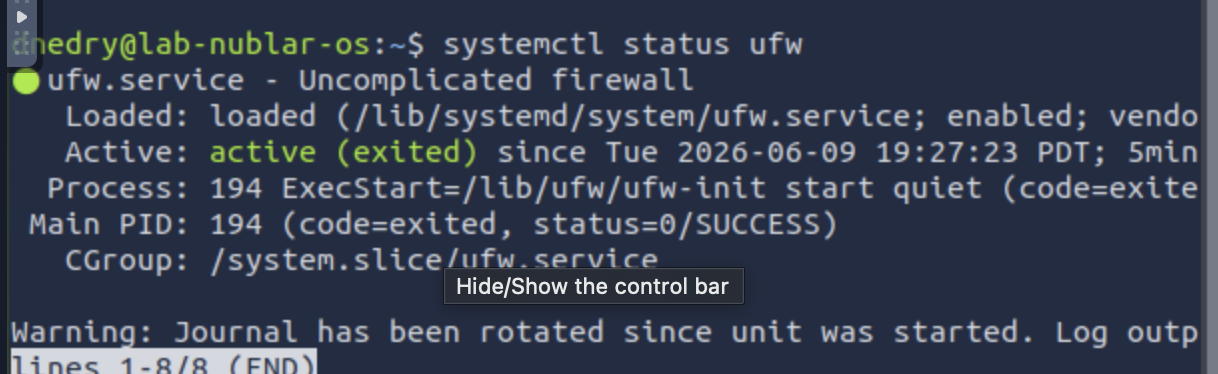
\includegraphics[width=0.6\textwidth]{firewall.png}
\end{center}

\subsubsection{4.6 Enumeración SUID}
Para proseguir buscamos los archivos del sistema que tienen permisos especiales para ejecutarse con los privilegios del propietario (que suele ser root) para la \textbf{escalada definitiva de privilegios}. Tenemos que encontrar qué archivos binarios con bit SUID activo existen en el sistema y encontramos esta \href{https://www.linuxtotal.com.mx/index.php?cont=info__tips_016}{guía} y esta \href{https://man7.org/linux/man-pages/man1/find.1.html}{oficial de Linux}.
\begin{lstlisting}[language=bash]
find / -perm -4000 -type f 2>/dev/null | wc -l
\end{lstlisting}
\begin{itemize}
    \item 16 archivos con bit SUID activo:
\end{itemize}
\begin{center}
    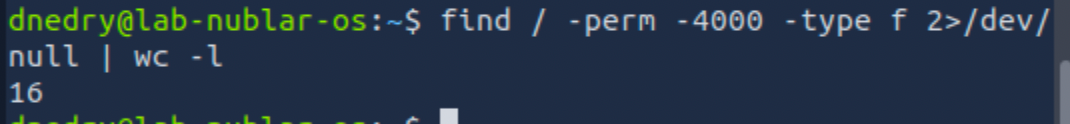
\includegraphics[width=0.55\textwidth]{image-61.png}
\end{center}

\subsubsection{4.7 Versión paquete apt}
Proseguimos buscando la versión del paquete \textbf{apt} para comprobar si el paquete es vulnerable a ataques conocidos (CVEs). Para ello tiramos de comandos encontrados en \href{https://blog.packagecloud.io/apt-cheat-sheet/#:~:text=Use%20the%20apt%2Dcache%20show,command%20to%20install%20a%20package.}{PackageCloud} y \href{https://askubuntu.com/questions/110123/how-do-i-find-a-list-of-packages-with-priority-required}{AskUbuntu}.
\begin{lstlisting}[language=bash]
apt-cache policy apt
dpkg-query -W -f='${Package}: ${Priority}\n' apt
\end{lstlisting}
\begin{itemize}
    \item apt tiene la versión 1.2.32ubuntu0.1 con prioridad \textbf{important}
\end{itemize}

\newpage

\subsection{05 - Fase de Escalada de Privilegios}
Tras obtener acceso inicial al sistema, la siguiente etapa de la auditoría se centró en la \textbf{escalada de privilegios}, cuyo objetivo es determinar si un usuario con permisos limitados puede alcanzar privilegios administrativos.

\subsubsection{5.1 Evaluación de controles de acceso: revisión de sudo y su}
Tratamos de cambiar de usuario con \texttt{su} pero nos retorna auth failure aun metiendo la contraseña intentando variaciones como root o user2, nos percatamos que hay que buscar un vector de ataque:
\begin{center}
    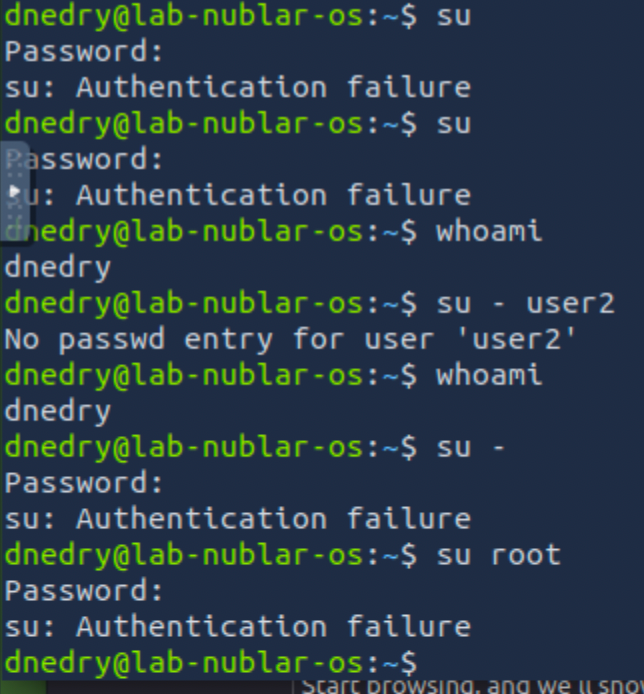
\includegraphics[width=0.55\textwidth]{image-64.png}
\end{center}
\begin{lstlisting}[language=bash]
su
\end{lstlisting}

Revisamos una \href{https://delinea.com/blog/linux-privilege-escalation}{guía de cómo hacer escalada de privilegios} y revisando comandos encontramos \texttt{sudo -l} que lista comandos que permiten \textbf{sudo}, para saltarnos la contraseña que nos da auth failure.
\begin{lstlisting}[language=bash]
sudo -l
\end{lstlisting}
\begin{itemize}
    \item Observamos que \texttt{tar} no requiere password:
\end{itemize}
\begin{center}
    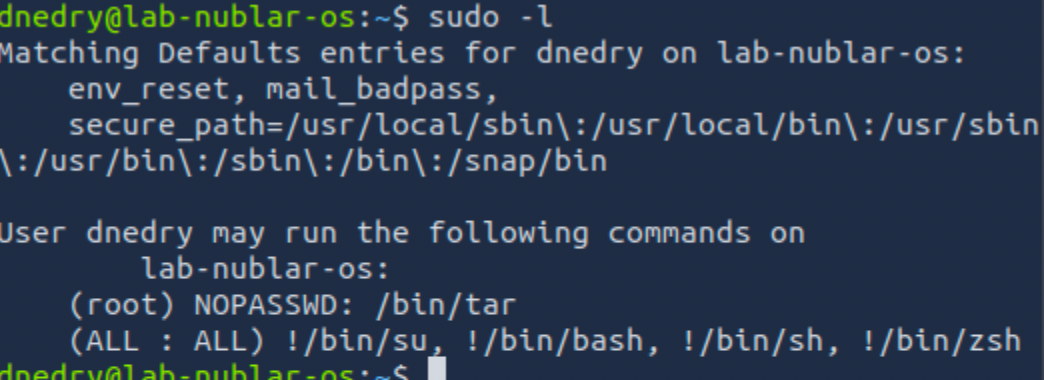
\includegraphics[width=0.65\textwidth]{image-65.png}
\end{center}

\subsubsection{5.2 Escalada mediante tar}
Buscamos en Google \textbf{"sudo -l" tar privilege escalation} y encontramos una \href{https://www.thehacker.recipes/infra/privilege-escalation/unix/sudo}{guía que nos ayuda con la escalada de privilegios a través de tar}.
Se detectó que el binario estándar de empaquetado \texttt{tar} se encontraba configurado con el bit SUID activo (permiso de ejecución de propietario asignado a root).
Abusando de las funcionalidades nativas de \texttt{tar}, se ejecutó una inyección de comandos aprovechando los parámetros de ejecución de checkpoints. Al procesar un archivo, el binario ejecutó una acción del sistema con los privilegios heredados de root.
\begin{lstlisting}[language=bash]
sudo /bin/tar -cf /dev/null /dev/null --checkpoint=1 --checkpoint-action=exec=/bin/sh
\end{lstlisting}
\begin{itemize}
    \item Obtención de root:
\end{itemize}
\begin{center}
    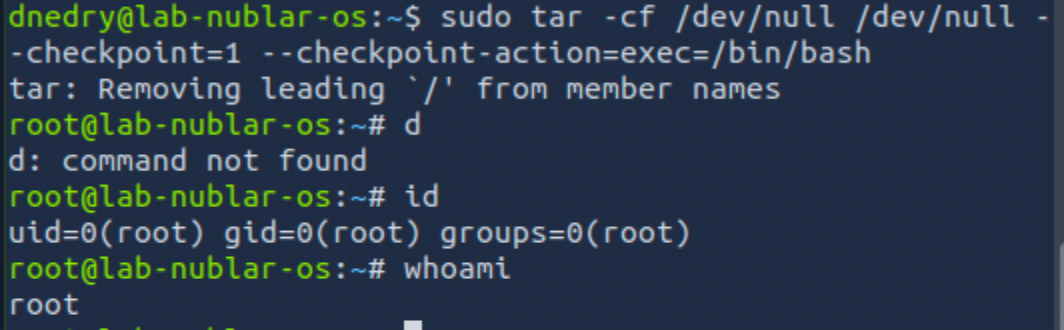
\includegraphics[width=0.6\textwidth]{image-66.png}
\end{center}

\begin{lstlisting}[language=bash]
id
% uid=0(root)
\end{lstlisting}

\begin{lstlisting}[language=bash]
cd /r00t
cat r00t.txt
\end{lstlisting}
La ejecución del comando anterior devolvió una shell interactiva con el identificador de usuario \textbf{uid=0(r00t)}. Con el control total de la máquina, se navega hacia el directorio personal del administrador para comprometer el objetivo final leyendo la flag del root:
\begin{center}
    
\includegraphics[width=0.30\textwidth]{image-69.png}
\end{center}

\subsubsection{5.4 Análisis Post-Explotación: Evaluación de controles de acceso}
Como no descubrimos qué nos devuelve la respuesta de qué pasa cuando se hace cambio de usuario hacemos un exit.
\begin{itemize}
    \item Hacemos \texttt{sudo su} para cambiar de usuario y al volver a root nos devuelve el mensaje que sucede al cambiar de usuario dándonos cuenta que no hacía falta hacer los pasos previos con \texttt{tar} para usar sudo ya que no requiere de contraseña:
\end{itemize}
\begin{center}
    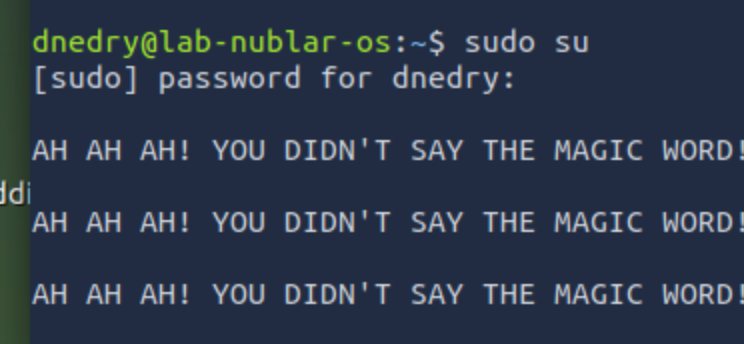
\includegraphics[width=0.30\textwidth]{image-68.png}
\end{center}

\subsubsection{5.5 Descifrado de IP ejecutora de procesos}
Para descubrir la IP que descubrió el proceso cogemos la \textbf{flag de root} y la desciframos con \href{https://elcodigoascii.com.ar/codigos-ascii/abre-llaves-curvas-codigo-ascii-123.html}{ASCII}.

\newpage

\subsection{06 - Conclusiones y Recomendaciones}
La auditoría del activo \textbf{lab-nublar-os} (10.130.135.78) confirma un escenario de riesgo crítico debido a la concatenación de dos fallos estructurales: exposición de backups en el servidor web (quiebra de \textbf{Confidencialidad}) y asignación laxa de permisos SUID/sudoers (quiebra de \textbf{Integridad}).

\textbf{Análisis de Riesgo Cuantitativo:} \\
La criticidad del activo se determina mediante la métrica estándar de gobernanza:

$$\text{Riesgo} = \text{Impacto} \times \text{Probabilidad}$$

\begin{itemize}
    \item \textbf{Impacto ($I$) - Crítico:} Compromiso total de la máquina (acceso root), lo cual conlleva pérdida de control de la infraestructura core, riesgo de exfiltración y parada de servicio (\textbf{Disponibilidad}).
    \item \textbf{Probabilidad ($P$) - Alta:} Vector inicial expuesto en el puerto 80. Explotación comun y tipica mediante técnicas automatizadas de reconocimiento (\textit{fuzzing}), sin requerir autenticación previa.
    \item \textbf{Resultado:} $\text{Crítico} \times \text{Alta} \rightarrow$ \textbf{Riesgo Global: Crítico}.
\end{itemize}

El plan de actuacion se integra bajo el modelo de mejora continua **PDCA** para pasar de una postura reactiva a una proactiva.

\vspace{0.4cm}

\textbf{Recomendaciones:}

\vspace{0.4cm}
\begin{table}[h!]
\centering
\small
\begin{tabular}{lll}
\toprule
\textbf{Prioridad} & \textbf{Acción de Remediación} & \textbf{Justificación Técnica} \\ \midrule
\textbf{Alta}  & \textbf{Limpieza de entorno} & Eliminar archivos \texttt{.bak} y \texttt{.zip} de directorios web. \\
\textbf{Alta}  & \textbf{Auditoría SUID} & Remover bit SUID de binarios no esenciales (\texttt{tar}, \texttt{find}). \\
\textbf{Alta}  & \textbf{Mínimo Privilegio} & Restringir permisos; asegurar acceso a lo estrictamente necesario. \\
\textbf{Media} & \textbf{Gestión de Credenciales} & Rotar llaves GPG/RSA y aplicar políticas robustas. \\
\textbf{Media} & \textbf{Hardening de Red} & Implementar segmentación mediante firewall para mitigar riesgos. \\
\textbf{Baja}  & \textbf{Trazabilidad y Logs} & Centralizar logs para asegurar la integridad de la autenticidad. \\ \bottomrule
\end{tabular}
\end{table}

\vspace{0.8cm}
\end{document}